\chapter{Mode~S enhanced surveillance}

Mode~S Enhanced Surveillance (EHS) provides a set of advanced functionalities for the Mode~S transponders. Three different types of reports are included in EHS. They are designed to report vertical intent, turning performance, and airspeeds. In this chapter, the structures and decoding processes of these reports are explained.

\section{Selected vertical intention (BDS 4,0)}

The selected vertical intention message is designed for air traffic control to obtain an aircraft's current vertical intentions. For example, an aircraft controller can use this information to check whether an aircraft is complying with an altitude command. 

Table \ref{tb:bds40} shows the structure of the message.

\begin{table}[ht]
\renewcommand{\arraystretch}{1.1}
\centering
\caption{Selected intention (BDS 4,0), MB field}
\label{tb:bds40}
\begin{tabular}{|l|l|l|l|}
\hline
\textbf{FIELD} & \textbf{MSG} & \textbf{MB} & \textbf{BITS} \\ \hline
Status (for MCP/FCU selected altitude) & 33 & 1 & 1 \\ \cdashline{1-1}
\begin{tabular}[c]{@{}l@{}}MCP/FCU selected altitude\\ Range: {[}0, 65520{]} ft\\ LSB: 16 ft\end{tabular} & 34-45 & 2-13 & 12 \\ \hline
Status (for FMS selected altitude) & 46 & 14 & 1 \\ \cdashline{1-1}
\begin{tabular}[c]{@{}l@{}}FMS selected altitude\\ Range: {[}0, 65520{]} ft\\ LSB: 16 ft\end{tabular} & 47-58 & 15-26 & 12 \\ \hline
Status (for barometric press setting) & 59 & 27 & 1 \\ \cdashline{1-1}
\begin{tabular}[c]{@{}l@{}}Barometric pressure setting\\ Note: actual value minus 800 mb\\ Range: {[}0, 410{]} mb\\ LSB: 0.1 mb\end{tabular} & 60-71 & 28-39 & 12 \\ \hline
Reserved (all zeros) & 72-79 & 40-47 & 8 \\ \hline
Status of MCP/FCU mode & 80 & 48 & 1 \\ \cdashline{1-1}
VNAV mode & 81 & 49 & 1 \\ \cdashline{1-1}
Alt hold mode & 82 & 50 & 1 \\ \cdashline{1-1}
Approach mode & 83 & 51 & 1 \\ \hline
Reserved (all zeros) & 84-85 & 52-53 & 2 \\ \hline
Status of target altitude source & 86 & 54 & 1 \\ \cdashline{1-1}
Target altitude source & 87-88 & 55-56 & 2 \\ \hline
\end{tabular}
\end{table}

Two different types of selected altitude fields are included in the message. Values in the \emph{MCP/FCU selected altitude} field are from the mode control panel or flight control unit. These are often inputs from the pilot. Values in \emph{FMS selected altitude} field are derived from the flight management system controlling the vertical profile, which often does not come from manual input.

The \emph{barometric pressure setting} value is the actual pressure in millibars (mb) subtracted by a constant of 800. If the actual value is below 800 mb (or above 1209 mb), the corresponding status bit (MB:27) is set to \0.

The last two bits in the MB field show the source of the target altitude. They have the following meaning:

\begin{verbatim}
  00: Unknown source
  01: Aircraft altitude
  10: FCU/MCP selected altitude
  11: FMS selected altitude
\end{verbatim}


In Figure \ref{fig:bds40_example}, an example of how to decode a BDS 4,0 message is illustrated:

\begin{figure}[ht]
  \centering
  

\tikzset{every picture/.style={line width=0.75pt}} %set default line width to 0.75pt        

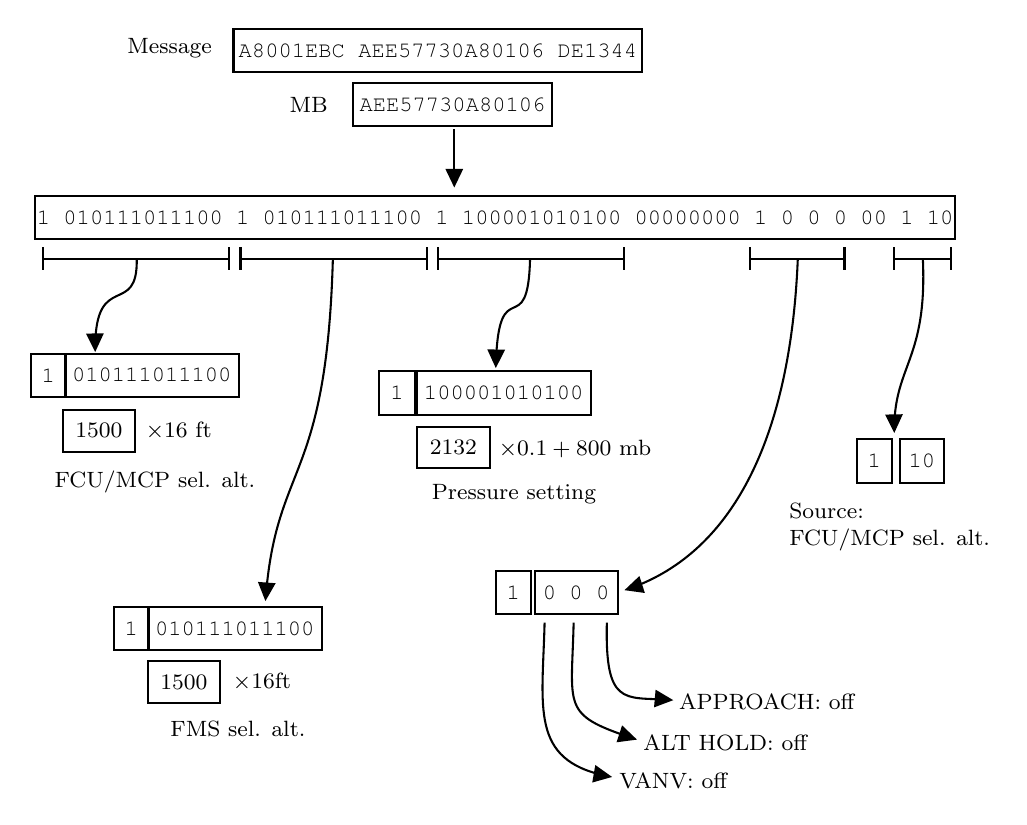
\begin{tikzpicture}[x=0.75pt,y=0.75pt,yscale=-1,xscale=1]
%uncomment if require: \path (0,432); %set diagram left start at 0, and has height of 432

%Curve Lines [id:da5981577463459831] 
\draw    (79,134.33) .. controls (79.57,162.77) and (59.38,139.8) .. (58.99,176.32) ;
\draw [shift={(59,179.25)}, rotate = 269.06] [fill={rgb, 255:red, 0; green, 0; blue, 0 }  ][line width=0.08]  [draw opacity=0] (8.93,-4.29) -- (0,0) -- (8.93,4.29) -- cycle    ;
%Curve Lines [id:da5084877796322058] 
\draw    (173.5,134.33) .. controls (170.45,242.9) and (146.49,231.49) .. (141.16,297.23) ;
\draw [shift={(141,299.25)}, rotate = 274.21] [fill={rgb, 255:red, 0; green, 0; blue, 0 }  ][line width=0.08]  [draw opacity=0] (8.93,-4.29) -- (0,0) -- (8.93,4.29) -- cycle    ;
%Curve Lines [id:da5650542056811212] 
\draw    (268.5,134.33) .. controls (267.52,175.49) and (253.57,139.5) .. (252.08,184.16) ;
\draw [shift={(252,187)}, rotate = 271.17] [fill={rgb, 255:red, 0; green, 0; blue, 0 }  ][line width=0.08]  [draw opacity=0] (8.93,-4.29) -- (0,0) -- (8.93,4.29) -- cycle    ;
%Curve Lines [id:da2826034018830037] 
\draw    (275.5,309.67) .. controls (274.52,350.62) and (268.32,375.72) .. (305.09,383.44) ;
\draw [shift={(308,384)}, rotate = 189.93] [fill={rgb, 255:red, 0; green, 0; blue, 0 }  ][line width=0.08]  [draw opacity=0] (8.93,-4.29) -- (0,0) -- (8.93,4.29) -- cycle    ;
%Curve Lines [id:da167001333387915] 
\draw    (289.5,309.67) .. controls (288.52,350.62) and (283.59,353.86) .. (317.33,365.12) ;
\draw [shift={(320,366)}, rotate = 198.12] [fill={rgb, 255:red, 0; green, 0; blue, 0 }  ][line width=0.08]  [draw opacity=0] (8.93,-4.29) -- (0,0) -- (8.93,4.29) -- cycle    ;
%Curve Lines [id:da03103602868349009] 
\draw    (305.5,309.67) .. controls (304.55,349.78) and (313.93,345.5) .. (334.51,346.78) ;
\draw [shift={(337.5,347)}, rotate = 185.04] [fill={rgb, 255:red, 0; green, 0; blue, 0 }  ][line width=0.08]  [draw opacity=0] (8.93,-4.29) -- (0,0) -- (8.93,4.29) -- cycle    ;
%Curve Lines [id:da5417401260605015] 
\draw    (457.75,134.33) .. controls (459.93,182.51) and (444.32,185.45) .. (443.99,215.39) ;
\draw [shift={(444,218.25)}, rotate = 268.83] [fill={rgb, 255:red, 0; green, 0; blue, 0 }  ][line width=0.08]  [draw opacity=0] (8.93,-4.29) -- (0,0) -- (8.93,4.29) -- cycle    ;
%Straight Lines [id:da924076364834967] 
\draw [line width=0.75]    (224,134.33) -- (313.6,134.33) ;
\draw [shift={(313.6,134.33)}, rotate = 180] [color={rgb, 255:red, 0; green, 0; blue, 0 }  ][line width=0.75]    (0,5.59) -- (0,-5.59)   ;
\draw [shift={(224,134.33)}, rotate = 180] [color={rgb, 255:red, 0; green, 0; blue, 0 }  ][line width=0.75]    (0,5.59) -- (0,-5.59)   ;
%Straight Lines [id:da1126730298431704] 
\draw [line width=0.75]    (129,134.33) -- (218.8,134.33) ;
\draw [shift={(218.8,134.33)}, rotate = 180] [color={rgb, 255:red, 0; green, 0; blue, 0 }  ][line width=0.75]    (0,5.59) -- (0,-5.59)   ;
\draw [shift={(129,134.33)}, rotate = 180] [color={rgb, 255:red, 0; green, 0; blue, 0 }  ][line width=0.75]    (0,5.59) -- (0,-5.59)   ;
%Straight Lines [id:da6889757950929192] 
\draw [line width=0.75]    (34,134.33) -- (123.6,134.33) ;
\draw [shift={(123.6,134.33)}, rotate = 180] [color={rgb, 255:red, 0; green, 0; blue, 0 }  ][line width=0.75]    (0,5.59) -- (0,-5.59)   ;
\draw [shift={(34,134.33)}, rotate = 180] [color={rgb, 255:red, 0; green, 0; blue, 0 }  ][line width=0.75]    (0,5.59) -- (0,-5.59)   ;
%Straight Lines [id:da5545710261355621] 
\draw [line width=0.75]    (374.5,134.33) -- (420,134.33) ;
\draw [shift={(420,134.33)}, rotate = 180] [color={rgb, 255:red, 0; green, 0; blue, 0 }  ][line width=0.75]    (0,5.59) -- (0,-5.59)   ;
\draw [shift={(374.5,134.33)}, rotate = 180] [color={rgb, 255:red, 0; green, 0; blue, 0 }  ][line width=0.75]    (0,5.59) -- (0,-5.59)   ;
%Straight Lines [id:da06655537350580443] 
\draw [line width=0.75]    (444,134.33) -- (471.5,134.33) ;
\draw [shift={(471.5,134.33)}, rotate = 180] [color={rgb, 255:red, 0; green, 0; blue, 0 }  ][line width=0.75]    (0,5.59) -- (0,-5.59)   ;
\draw [shift={(444,134.33)}, rotate = 180] [color={rgb, 255:red, 0; green, 0; blue, 0 }  ][line width=0.75]    (0,5.59) -- (0,-5.59)   ;
%Curve Lines [id:da6196785513080374] 
\draw    (397.5,134.33) .. controls (394.13,217.73) and (367.81,275.25) .. (316.37,293.21) ;
\draw [shift={(314,294)}, rotate = 342.22] [fill={rgb, 255:red, 0; green, 0; blue, 0 }  ][line width=0.08]  [draw opacity=0] (8.93,-4.29) -- (0,0) -- (8.93,4.29) -- cycle    ;
%Straight Lines [id:da65120732921535] 
\draw    (232,72) -- (232,97) ;
\draw [shift={(232,100)}, rotate = 270] [fill={rgb, 255:red, 0; green, 0; blue, 0 }  ][line width=0.08]  [draw opacity=0] (8.93,-4.29) -- (0,0) -- (8.93,4.29) -- cycle    ;

% Text Node
\draw    (125.63,23.5) -- (322.63,23.5) -- (322.63,44.5) -- (125.63,44.5) -- cycle  ;
\draw (224.13,34) node  [font=\footnotesize] [align=left] {{\fontfamily{pcr}\selectfont A8001EBC AEE57730A80106 DE1344}};
% Text Node
\draw (161.88,60) node  [font=\footnotesize] [align=left] {MB};
% Text Node
\draw    (30.2,104) -- (473.2,104) -- (473.2,125) -- (30.2,125) -- cycle  ;
\draw (251.7,114.5) node  [font=\footnotesize] [align=left] {{\fontfamily{pcr}\selectfont 1 010111011100 1 010111011100 1 100001010100 00000000 1 0 0 0 00 1 10}};
% Text Node
\draw    (183.13,49.5) -- (279.13,49.5) -- (279.13,70.5) -- (183.13,70.5) -- cycle  ;
\draw (231.13,60) node  [font=\footnotesize] [align=left] {{\fontfamily{pcr}\selectfont AEE57730A80106}};
% Text Node
\draw    (27.88,180) -- (44.88,180) -- (44.88,201) -- (27.88,201) -- cycle  ;
\draw (36.38,190.5) node  [font=\footnotesize] [align=left] {{\fontfamily{pcr}\selectfont 1}};
% Text Node
\draw    (44.26,180) -- (128.26,180) -- (128.26,201) -- (44.26,201) -- cycle  ;
\draw (86.26,190.5) node  [font=\footnotesize] [align=left] {{\fontfamily{pcr}\selectfont 010111011100}};
% Text Node
\draw    (43.26,207.25) -- (78.26,207.25) -- (78.26,227.25) -- (43.26,227.25) -- cycle  ;
\draw (60.76,217.25) node  [font=\footnotesize] [align=left] {1500};
% Text Node
\draw (81.87,217.25) node [anchor=west] [inner sep=0.75pt]  [font=\footnotesize] [align=left] {$\displaystyle \times 16$ ft};
% Text Node
\draw    (67.88,302) -- (84.88,302) -- (84.88,323) -- (67.88,323) -- cycle  ;
\draw (76.38,312.5) node  [font=\footnotesize] [align=left] {{\fontfamily{pcr}\selectfont 1}};
% Text Node
\draw    (84.26,302) -- (168.26,302) -- (168.26,323) -- (84.26,323) -- cycle  ;
\draw (126.26,312.5) node  [font=\footnotesize] [align=left] {{\fontfamily{pcr}\selectfont 010111011100}};
% Text Node
\draw    (84.26,328.25) -- (119.26,328.25) -- (119.26,348.25) -- (84.26,348.25) -- cycle  ;
\draw (101.76,338.25) node  [font=\footnotesize] [align=left] {1500};
% Text Node
\draw (123.87,338.25) node [anchor=west] [inner sep=0.75pt]  [font=\footnotesize] [align=left] {$\displaystyle \times 16${\fontfamily{pcr}\selectfont  }ft};
% Text Node
\draw    (195.88,188.5) -- (212.88,188.5) -- (212.88,209.5) -- (195.88,209.5) -- cycle  ;
\draw (204.38,199) node  [font=\footnotesize] [align=left] {{\fontfamily{pcr}\selectfont 1}};
% Text Node
\draw    (213.8,188.5) -- (297.8,188.5) -- (297.8,209.5) -- (213.8,209.5) -- cycle  ;
\draw (255.8,199) node  [font=\footnotesize] [align=left] {{\fontfamily{pcr}\selectfont 100001010100}};
% Text Node
\draw    (214.1,215.25) -- (249.1,215.25) -- (249.1,235.25) -- (214.1,235.25) -- cycle  ;
\draw (231.6,225.25) node  [font=\footnotesize] [align=left] {2132};
% Text Node
\draw (252,225.75) node [anchor=west] [inner sep=0.75pt]  [font=\footnotesize] [align=left] {$\displaystyle \times 0.1+800$ mb};
% Text Node
\draw (94.82,33) node  [font=\footnotesize] [align=left] {Message};
% Text Node
\draw    (425.88,221.33) -- (442.88,221.33) -- (442.88,242.33) -- (425.88,242.33) -- cycle  ;
\draw (434.38,231.83) node  [font=\footnotesize] [align=left] {{\fontfamily{pcr}\selectfont 1}};
% Text Node
\draw    (446.8,221.33) -- (467.8,221.33) -- (467.8,242.33) -- (446.8,242.33) -- cycle  ;
\draw (457.3,231.83) node  [font=\footnotesize] [align=left] {{\fontfamily{pcr}\selectfont 10}};
% Text Node
\draw    (251.88,284.67) -- (268.88,284.67) -- (268.88,305.67) -- (251.88,305.67) -- cycle  ;
\draw (260.38,295.17) node  [font=\footnotesize] [align=left] {{\fontfamily{pcr}\selectfont 1}};
% Text Node
\draw    (270.7,284.67) -- (310.7,284.67) -- (310.7,305.67) -- (270.7,305.67) -- cycle  ;
\draw (290.7,295.17) node  [font=\footnotesize] [align=left] {{\fontfamily{pcr}\selectfont 0 0 0}};
% Text Node
\draw (337.45,385.67) node  [font=\footnotesize] [align=left] {VANV: off};
% Text Node
\draw (362.53,367.33) node  [font=\footnotesize] [align=left] {ALT HOLD: off};
% Text Node
\draw (382.53,347.67) node  [font=\footnotesize] [align=left] {APPROACH: off};
% Text Node
\draw (441.76,263.67) node  [font=\footnotesize] [align=left] {Source:\\FCU/MCP sel. alt.};
% Text Node
\draw (87.76,241.67) node  [font=\footnotesize] [align=left] {FCU/MCP sel. alt.};
% Text Node
\draw (127.76,360.67) node  [font=\footnotesize] [align=left] {FMS sel. alt.};
% Text Node
\draw (260.76,247.67) node  [font=\footnotesize] [align=left] {Pressure setting};


\end{tikzpicture}

  \vspace{0.2cm}
  \caption{BDS 4,0 decoding example}
  \label{fig:bds40_example}
\end{figure}

\begin{notebox}{Try it out}
Using \texttt{pyModeS}, we can decode information of BDS 4,0 messages as: 

\begin{verbatim}
import pyModeS as pms

msg = "A8001EBCAEE57730A80106DE1344"
selaltfms = pms.commb.selalt40fms(msg)
selaltmcp = pms.commb.selalt40mcp(msg)
pressure = pms.commb.p40baro(msg)
\end{verbatim}

\end{notebox}



\clearpage

\section{Track and turn report (BDS 5,0)}

The track and turn report is designed to provide parameters to describe aircraft turns. In this type of message, roll angle, track angle, and track rate are provided. It also includes the ground speed and true airspeed (TAS) of the aircraft.

Table \ref{tb:bds50} shows the structure of the message.

\begin{table}[ht]
\renewcommand{\arraystretch}{1.1}
\centering
\caption{Track and turn report (BDS 5,0), MB field}
\label{tb:bds50}
\begin{tabular}{|l|l|l|l|}
\hline
\textbf{FIELD} & \textbf{MSG} & \textbf{MB} & \textbf{BITS} \\ \hline
Status (for roll angle) & 33 & 1 & 1 \\ \cdashline{1-1}
Sign & 34 & 2 & 1 \\ \cdashline{1-1}
\begin{tabular}[c]{@{}l@{}}Roll angle\\ Range: {[}-90, +90{]} degrees\\ LSB: 45/256 degrees\end{tabular} & 35-43 & 3-11 & 9 \\ \hline
Status (for track angle) & 44 & 12 & 1 \\ \cdashline{1-1}
Sign & 45 & 13 & 1 \\ \cdashline{1-1}
\begin{tabular}[c]{@{}l@{}}True track angle\\ Range: {[}-180, 180{]} degrees\\ LSB: 90/512 degrees\end{tabular} & 46-55 & 14-23 & 10 \\ \hline
Status (for ground speed) & 56 & 24 & 1 \\ \cdashline{1-1}
\begin{tabular}[c]{@{}l@{}}Ground speed\\ Range: {[}0, 2046{]} kt\\ LSB: 2 kt\end{tabular} & 57-66 & 25-34 & 10 \\ \hline
Status (for track angle rate) & 67 & 35 & 1 \\ \cdashline{1-1}
Sign & 68 & 36 & 1 \\ \cdashline{1-1}
\begin{tabular}[c]{@{}l@{}}Track angle rate\\ Range: {[}-16, 16{]} degrees/second\\ LSB: 8/256 degrees/second\end{tabular} & 69-77 & 37-45 & 9 \\ \hline
Status (for true airspeed) & 78 & 46 & 1 \\ \cdashline{1-1}
\begin{tabular}[c]{@{}l@{}}True airspeed\\ Range: {[}0, 2046{]} kt\\ LSB: 2 kt\end{tabular} & 79-88 & 47-56 & 10 \\ \hline
\end{tabular}
\end{table}

In this message, we can see three signed values, which are roll angle, track angle, and track angle rate. Two's complement coding (see section \ref{sec:two_complement}) should be used to calculate these values.

In Figure \ref{fig:bds50_example}, an example of how to decode a BDS 5,0 message is illustrated.

\begin{figure}[ht]
  \centering
  

\tikzset{every picture/.style={line width=0.75pt}} %set default line width to 0.75pt        

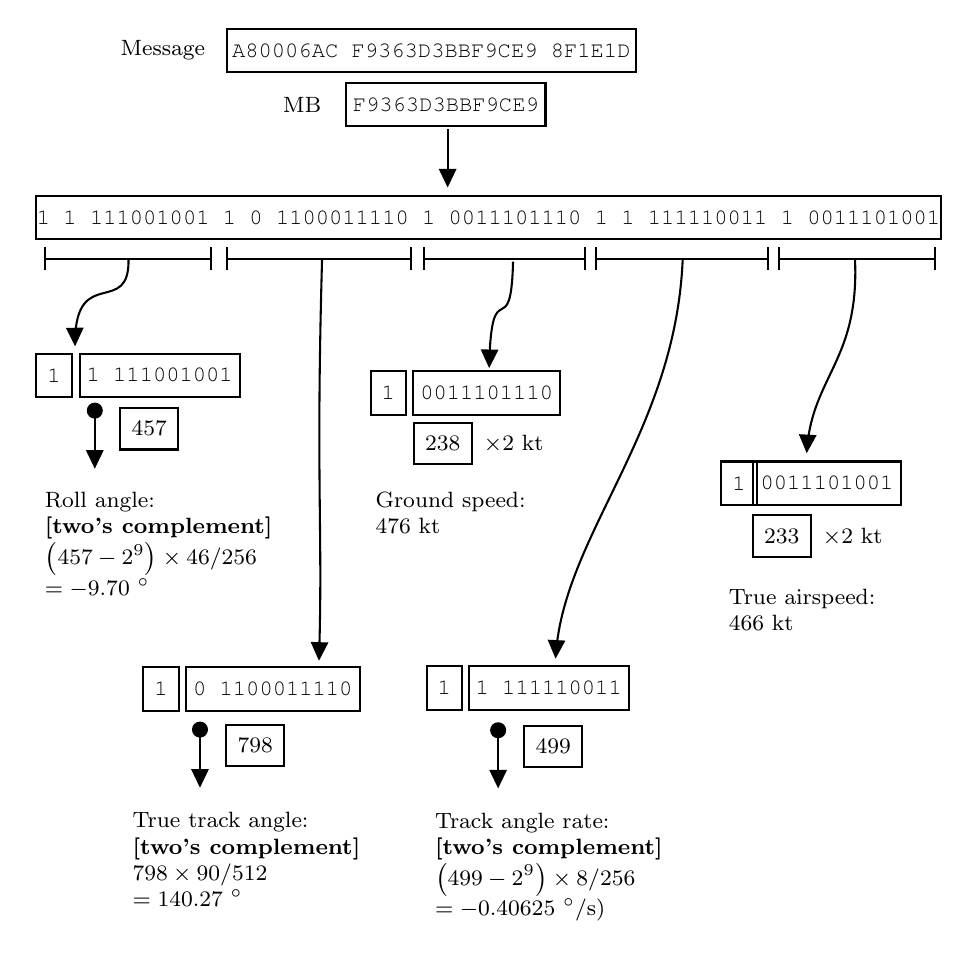
\begin{tikzpicture}[x=0.75pt,y=0.75pt,yscale=-1,xscale=1]
%uncomment if require: \path (0,537); %set diagram left start at 0, and has height of 537

%Curve Lines [id:da05193136470258586] 
\draw    (78.25,134.33) .. controls (78.82,162.77) and (53.17,137.18) .. (52.5,173.58) ;
\draw [shift={(52.5,176.5)}, rotate = 269.06] [fill={rgb, 255:red, 0; green, 0; blue, 0 }  ][line width=0.08]  [draw opacity=0] (8.93,-4.29) -- (0,0) -- (8.93,4.29) -- cycle    ;
%Curve Lines [id:da42930744707627944] 
\draw    (171.5,134.33) .. controls (168.46,242.36) and (171.89,264.35) .. (170.09,325.19) ;
\draw [shift={(170,328)}, rotate = 271.82] [fill={rgb, 255:red, 0; green, 0; blue, 0 }  ][line width=0.08]  [draw opacity=0] (8.93,-4.29) -- (0,0) -- (8.93,4.29) -- cycle    ;
%Curve Lines [id:da6810825834819927] 
\draw    (263.5,135.75) .. controls (262.52,176.91) and (253.38,139.56) .. (252.07,184.17) ;
\draw [shift={(252,187)}, rotate = 271.17] [fill={rgb, 255:red, 0; green, 0; blue, 0 }  ][line width=0.08]  [draw opacity=0] (8.93,-4.29) -- (0,0) -- (8.93,4.29) -- cycle    ;
%Curve Lines [id:da02210524649932588] 
\draw    (428.25,134.33) .. controls (430.44,182.76) and (408.16,190.62) .. (405.19,225.28) ;
\draw [shift={(405,228)}, rotate = 273.09000000000003] [fill={rgb, 255:red, 0; green, 0; blue, 0 }  ][line width=0.08]  [draw opacity=0] (8.93,-4.29) -- (0,0) -- (8.93,4.29) -- cycle    ;
%Straight Lines [id:da8287402060207048] 
\draw [line width=0.75]    (220.5,134.33) -- (298,134.33) ;
\draw [shift={(298,134.33)}, rotate = 180] [color={rgb, 255:red, 0; green, 0; blue, 0 }  ][line width=0.75]    (0,5.59) -- (0,-5.59)   ;
\draw [shift={(220.5,134.33)}, rotate = 180] [color={rgb, 255:red, 0; green, 0; blue, 0 }  ][line width=0.75]    (0,5.59) -- (0,-5.59)   ;
%Straight Lines [id:da6940086335708118] 
\draw [line width=0.75]    (125.5,134.33) -- (214.5,134.33) ;
\draw [shift={(214.5,134.33)}, rotate = 180] [color={rgb, 255:red, 0; green, 0; blue, 0 }  ][line width=0.75]    (0,5.59) -- (0,-5.59)   ;
\draw [shift={(125.5,134.33)}, rotate = 180] [color={rgb, 255:red, 0; green, 0; blue, 0 }  ][line width=0.75]    (0,5.59) -- (0,-5.59)   ;
%Straight Lines [id:da5605080029920126] 
\draw [line width=0.75]    (38,134.33) -- (118,134.33) ;
\draw [shift={(118,134.33)}, rotate = 180] [color={rgb, 255:red, 0; green, 0; blue, 0 }  ][line width=0.75]    (0,5.59) -- (0,-5.59)   ;
\draw [shift={(38,134.33)}, rotate = 180] [color={rgb, 255:red, 0; green, 0; blue, 0 }  ][line width=0.75]    (0,5.59) -- (0,-5.59)   ;
%Straight Lines [id:da26733404149104456] 
\draw [line width=0.75]    (303.5,134.33) -- (386.4,134.33) ;
\draw [shift={(386.4,134.33)}, rotate = 180] [color={rgb, 255:red, 0; green, 0; blue, 0 }  ][line width=0.75]    (0,5.59) -- (0,-5.59)   ;
\draw [shift={(303.5,134.33)}, rotate = 180] [color={rgb, 255:red, 0; green, 0; blue, 0 }  ][line width=0.75]    (0,5.59) -- (0,-5.59)   ;
%Straight Lines [id:da42135663368948384] 
\draw [line width=0.75]    (391.5,134.33) -- (467,134.33) ;
\draw [shift={(467,134.33)}, rotate = 180] [color={rgb, 255:red, 0; green, 0; blue, 0 }  ][line width=0.75]    (0,5.59) -- (0,-5.59)   ;
\draw [shift={(391.5,134.33)}, rotate = 180] [color={rgb, 255:red, 0; green, 0; blue, 0 }  ][line width=0.75]    (0,5.59) -- (0,-5.59)   ;
%Curve Lines [id:da9172630037641052] 
\draw    (345.25,134.33) .. controls (341.88,217.73) and (288.63,266.52) .. (284.17,324.35) ;
\draw [shift={(284,327)}, rotate = 272.90999999999997] [fill={rgb, 255:red, 0; green, 0; blue, 0 }  ][line width=0.08]  [draw opacity=0] (8.93,-4.29) -- (0,0) -- (8.93,4.29) -- cycle    ;
%Straight Lines [id:da508696319168084] 
\draw    (232,72) -- (232,97) ;
\draw [shift={(232,100)}, rotate = 270] [fill={rgb, 255:red, 0; green, 0; blue, 0 }  ][line width=0.08]  [draw opacity=0] (8.93,-4.29) -- (0,0) -- (8.93,4.29) -- cycle    ;
%Straight Lines [id:da38703610180504544] 
\draw    (62,207.5) -- (62,232.5) ;
\draw [shift={(62,235.5)}, rotate = 270] [fill={rgb, 255:red, 0; green, 0; blue, 0 }  ][line width=0.08]  [draw opacity=0] (8.93,-4.29) -- (0,0) -- (8.93,4.29) -- cycle    ;
\draw [shift={(62,207.5)}, rotate = 90] [color={rgb, 255:red, 0; green, 0; blue, 0 }  ][fill={rgb, 255:red, 0; green, 0; blue, 0 }  ][line width=0.75]      (0, 0) circle [x radius= 3.35, y radius= 3.35]   ;
%Straight Lines [id:da8199855675170937] 
\draw    (112.67,361.17) -- (112.67,386.17) ;
\draw [shift={(112.67,389.17)}, rotate = 270] [fill={rgb, 255:red, 0; green, 0; blue, 0 }  ][line width=0.08]  [draw opacity=0] (8.93,-4.29) -- (0,0) -- (8.93,4.29) -- cycle    ;
\draw [shift={(112.67,361.17)}, rotate = 90] [color={rgb, 255:red, 0; green, 0; blue, 0 }  ][fill={rgb, 255:red, 0; green, 0; blue, 0 }  ][line width=0.75]      (0, 0) circle [x radius= 3.35, y radius= 3.35]   ;
%Straight Lines [id:da9593907742960721] 
\draw    (256.33,361.5) -- (256.33,386.5) ;
\draw [shift={(256.33,389.5)}, rotate = 270] [fill={rgb, 255:red, 0; green, 0; blue, 0 }  ][line width=0.08]  [draw opacity=0] (8.93,-4.29) -- (0,0) -- (8.93,4.29) -- cycle    ;
\draw [shift={(256.33,361.5)}, rotate = 90] [color={rgb, 255:red, 0; green, 0; blue, 0 }  ][fill={rgb, 255:red, 0; green, 0; blue, 0 }  ][line width=0.75]      (0, 0) circle [x radius= 3.35, y radius= 3.35]   ;

% Text Node
\draw    (125.63,23.5) -- (322.63,23.5) -- (322.63,44.5) -- (125.63,44.5) -- cycle  ;
\draw (224.13,34) node  [font=\footnotesize] [align=left] {{\fontfamily{pcr}\selectfont A80006AC F9363D3BBF9CE9 8F1E1D}};
% Text Node
\draw (161.88,60) node  [font=\footnotesize] [align=left] {MB};
% Text Node
\draw    (33.7,104) -- (469.7,104) -- (469.7,125) -- (33.7,125) -- cycle  ;
\draw (251.7,114.5) node  [font=\footnotesize] [align=left] {{\fontfamily{pcr}\selectfont 1 1 111001001 1 0 1100011110 1 0011101110 1 1 111110011 1 0011101001}};
% Text Node
\draw    (183.13,49.5) -- (279.13,49.5) -- (279.13,70.5) -- (183.13,70.5) -- cycle  ;
\draw (231.13,60) node  [font=\footnotesize] [align=left] {{\fontfamily{pcr}\selectfont F9363D3BBF9CE9}};
% Text Node
\draw    (33.88,180) -- (50.88,180) -- (50.88,201) -- (33.88,201) -- cycle  ;
\draw (42.38,190.5) node  [font=\footnotesize] [align=left] {{\fontfamily{pcr}\selectfont 1}};
% Text Node
\draw    (54.76,180) -- (131.76,180) -- (131.76,201) -- (54.76,201) -- cycle  ;
\draw (93.26,190.5) node  [font=\footnotesize] [align=left] {{\fontfamily{pcr}\selectfont 1 111001001}};
% Text Node
\draw    (74.26,206.25) -- (102.26,206.25) -- (102.26,226.25) -- (74.26,226.25) -- cycle  ;
\draw (88.26,216.25) node  [font=\footnotesize] [align=left] {457};
% Text Node
\draw    (85.38,331) -- (102.38,331) -- (102.38,352) -- (85.38,352) -- cycle  ;
\draw (93.88,341.5) node  [font=\footnotesize] [align=left] {{\fontfamily{pcr}\selectfont 1}};
% Text Node
\draw    (105.76,331) -- (189.76,331) -- (189.76,352) -- (105.76,352) -- cycle  ;
\draw (147.76,341.5) node  [font=\footnotesize] [align=left] {{\fontfamily{pcr}\selectfont 0 1100011110}};
% Text Node
\draw    (125.26,358.92) -- (153.26,358.92) -- (153.26,378.92) -- (125.26,378.92) -- cycle  ;
\draw (139.26,368.92) node  [font=\footnotesize] [align=left] {798};
% Text Node
\draw    (194.88,188.5) -- (211.88,188.5) -- (211.88,209.5) -- (194.88,209.5) -- cycle  ;
\draw (203.38,199) node  [font=\footnotesize] [align=left] {{\fontfamily{pcr}\selectfont 1}};
% Text Node
\draw    (215.3,188.5) -- (286.3,188.5) -- (286.3,209.5) -- (215.3,209.5) -- cycle  ;
\draw (250.8,199) node  [font=\footnotesize] [align=left] {{\fontfamily{pcr}\selectfont 0011101110}};
% Text Node
\draw    (215.6,213.25) -- (243.6,213.25) -- (243.6,233.25) -- (215.6,233.25) -- cycle  ;
\draw (229.6,223.25) node  [font=\footnotesize] [align=left] {238};
% Text Node
\draw (248,223.75) node [anchor=west] [inner sep=0.75pt]  [font=\footnotesize] [align=left] {$\displaystyle \times 2$ kt};
% Text Node
\draw (94.82,34) node  [font=\footnotesize] [align=left] {Message};
% Text Node
\draw    (363.88,232) -- (380.88,232) -- (380.88,253) -- (363.88,253) -- cycle  ;
\draw (372.38,242.5) node  [font=\footnotesize] [align=left] {{\fontfamily{pcr}\selectfont 1}};
% Text Node
\draw    (379.3,232) -- (450.3,232) -- (450.3,253) -- (379.3,253) -- cycle  ;
\draw (414.8,242.5) node  [font=\footnotesize] [align=left] {{\fontfamily{pcr}\selectfont 0011101001}};
% Text Node
\draw    (221.88,330.67) -- (238.88,330.67) -- (238.88,351.67) -- (221.88,351.67) -- cycle  ;
\draw (230.38,341.17) node  [font=\footnotesize] [align=left] {{\fontfamily{pcr}\selectfont 1}};
% Text Node
\draw    (242.2,330.67) -- (319.2,330.67) -- (319.2,351.67) -- (242.2,351.67) -- cycle  ;
\draw (280.7,341.17) node  [font=\footnotesize] [align=left] {{\fontfamily{pcr}\selectfont 1 111110011}};
% Text Node
\draw (92.76,272.17) node  [font=\footnotesize] [align=left] {Roll angle:\\\textbf{[two's complement]}\\$\displaystyle \left( 457-2^{9}\right) \times 46/256$\\$\displaystyle =-9.70\ ^{\circ }$};
% Text Node
\draw (233.42,256.67) node  [font=\footnotesize] [align=left] {Ground speed:\\476 kt};
% Text Node
\draw (135.09,423.83) node  [font=\footnotesize] [align=left] {True track angle:\\\textbf{[two's complement]}\\$\displaystyle 798\times 90/512$\\$\displaystyle =140.27\ ^{\circ }$};
% Text Node
\draw    (268.92,359.25) -- (296.92,359.25) -- (296.92,379.25) -- (268.92,379.25) -- cycle  ;
\draw (282.92,369.25) node  [font=\footnotesize] [align=left] {499};
% Text Node
\draw (280.76,427.5) node  [font=\footnotesize] [align=left] {Track angle rate:\\\textbf{[two's complement]}\\$\displaystyle \left( 499-2^{9}\right) \times 8/256$\\$\displaystyle =-0.40625\ ^{\circ }$/s)};
% Text Node
\draw    (378.93,257.92) -- (406.93,257.92) -- (406.93,277.92) -- (378.93,277.92) -- cycle  ;
\draw (392.93,267.92) node  [font=\footnotesize] [align=left] {233};
% Text Node
\draw (411.33,268.42) node [anchor=west] [inner sep=0.75pt]  [font=\footnotesize] [align=left] {$\displaystyle \times 2$ kt};
% Text Node
\draw (402.76,303.33) node  [font=\footnotesize] [align=left] {True airspeed:\\466 kt };


\end{tikzpicture}
  \vspace{0.5cm}
  \caption{BDS 5,0 decoding example}
  \label{fig:bds50_example}
\end{figure}

\begin{notebox}{Try it out}
Using \texttt{pyModeS}, we can decode information of BDS 5,0 messages as: 

\begin{verbatim}
import pyModeS as pms

msg = "A80006ACF9363D3BBF9CE98F1E1D"

roll_angle = pms.commb.roll50(msg)
track_angle = pms.commb.trk50(msg)
track_angle_rate = pms.commb.rtrk50(msg)
ground_speed = pms.commb.gs50(msg)
TAS = pms.commb.tas50(msg)
\end{verbatim}

\end{notebox}


\clearpage

\section{Heading and speed report (BDS 6,0)}

The heading and speed report is designed to downlink various airspeed and vertical rate to air traffic controllers. In this type of message, indicated airspeed (IAS), Mach number, barometric altitude rate, inertial vertical velocity, and the magnetic heading of the aircraft are provided.

Table \ref{tb:bds60} shows the structure of the message.


\begin{table}[ht]
\renewcommand{\arraystretch}{1.1}
\centering
\caption{Heading and speed report (BDS 6,0), MB field}
\label{tb:bds60}
\begin{tabular}{|l|l|l|l|}
\hline
\textbf{FIELD} & \textbf{MSG} & \textbf{MB} & \textbf{BITS} \\ \hline
Status (for magnetic heading) & 33 & 1 & 1 \\ \cdashline{1-1}
Sign & 34 & 2 & 1 \\ \cdashline{1-1}
\begin{tabular}[c]{@{}l@{}}Magnetic heading\\ Range: {[}-180, +180{]} degrees\\ LSB: 90/512 degrees\end{tabular} & 35-44 & 3-12 & 10 \\ \hline
Status (for indicated airspeed) & 45 & 13 & 1 \\ \cdashline{1-1}
\begin{tabular}[c]{@{}l@{}}Indicated airspeed\\ Range: {[}0, 1023{]} kt\\ LSB: 1 kt\end{tabular} & 46-55 & 14-23 & 10 \\ \hline
Status (for Mach number) & 56 & 24 & 1 \\ \cdashline{1-1}
\begin{tabular}[c]{@{}l@{}}Mach number\\ Range: {[}0, 4.092{]}\\ LSB: 0.004\end{tabular} & 57-66 & 25-34 & 10 \\ \hline
Status (for barometric altitude rate) & 67 & 35 & 1 \\ \cdashline{1-1}
Sign & 68 & 36 & 1 \\ \cdashline{1-1}
\begin{tabular}[c]{@{}l@{}}Barometric altitude rate\\ Range: {[}-16384, +16352{]} ft/min\\ LSB: 32 ft/min\end{tabular} & 69-77 & 37-45 & 9 \\ \hline
Status (for inertial vertical velocity) & 78 & 46 & 1 \\ \cdashline{1-1}
Sign & 79 & 47 & 1 \\ \cdashline{1-1}
\begin{tabular}[c]{@{}l@{}}Inertial vertical velocity\\ Range: {[}-16384, +16352{]} ft/min\\ LSB: 32 ft/min\end{tabular} & 80-88 & 48-56 & 9 \\ \hline
\end{tabular}
\end{table}

In this message, we can see a few signed values, such as heading and two vertical rates. Two's complement coding (see section \ref{sec:two_complement}) should be used to calculate these values.

The magnetic heading is the aircraft's heading in respect to the magnetic North, which can be different from the true north (for example, used for the track angle from ADS-B and BDS 5,0). Often an aircraft obtains the magnetic heading by adding its true North heading with the magnetic declination from a world magnetic model, such as \cite{chulliat2015}. It is worth noting that the true North heading is not necessarily the same as the track angle due to the influence of wind.

In the heading and speed report, two different kinds of vertical rates are reported. Barometric altitude rates are only derived from barometer measurements. Due to the lacking of filtering from air data input, significant noise is contained in these values. On the other hand, inertial vertical velocities are values provided by navigational equipment from different sources including the flight management computer. According to \cite{icao9688}, data sources with different levels of priorities are defined for these two values, which are listed in Table \ref{tb:vertical_rate_source}.

\begin{table}[ht]
\footnotesize
\centering
\caption{Data sources for two vertical rates in heading and speed report}
\label{tb:vertical_rate_source}
\begin{tabular}{|l|l|}
\hline
\textbf{Parameter} & \textbf{Input Data Source Priorities} \\ \hline
Barometric altitude rate & \begin{tabular}[c]{@{}l@{}}1. Air Data System\\ 2. Inertial Reference System / Flight Management System\end{tabular} \\ \hline
Inertial vertical velocity & \begin{tabular}[c]{@{}l@{}}1. Flight Management Computer / GNSS integrated\\ 2. Flight Management Computer (General)\\ 3. Inertial Reference System / Flight Management System\end{tabular} \\ \hline
\end{tabular}
\end{table}


In Figure \ref{fig:bds60_example}, the example on how to decode a BDS 6,0 message is illustrated.

\begin{figure}[ht]
  \centering
  


\tikzset{every picture/.style={line width=0.75pt}} %set default line width to 0.75pt        

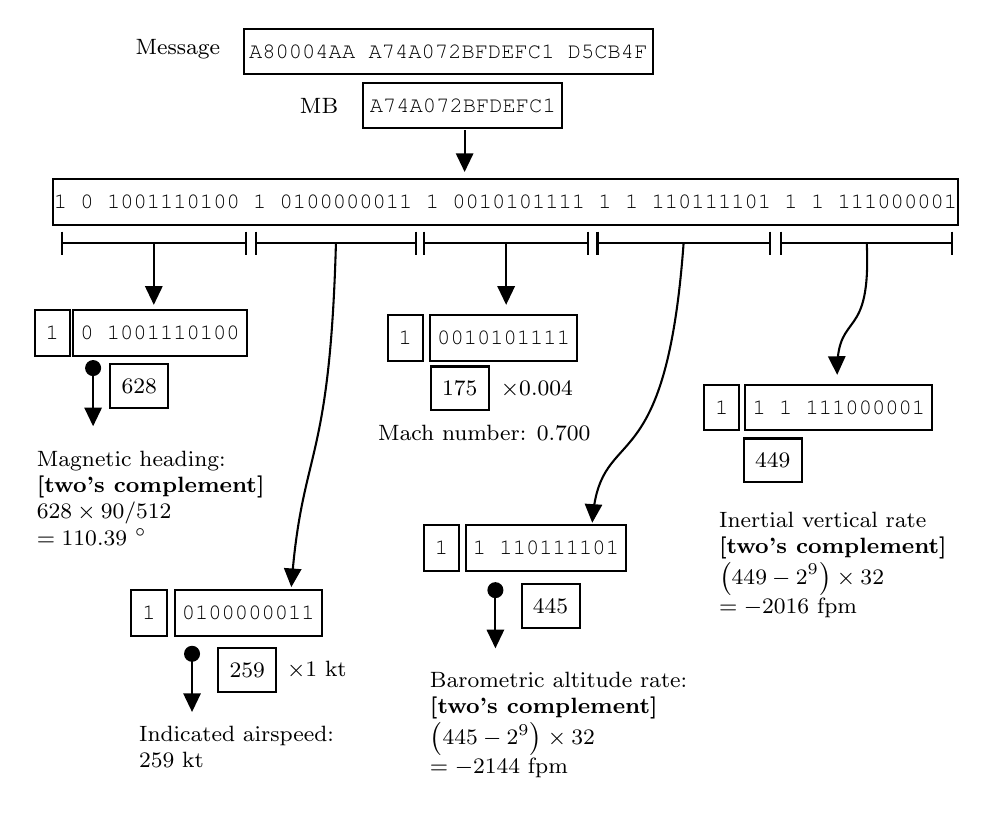
\begin{tikzpicture}[x=0.75pt,y=0.75pt,yscale=-1,xscale=1]
%uncomment if require: \path (0,574); %set diagram left start at 0, and has height of 574

%Curve Lines [id:da7633195255793686] 
\draw    (170,136.33) .. controls (166.95,244.9) and (153.77,234.23) .. (148.65,299.98) ;
\draw [shift={(148.5,302)}, rotate = 274.21] [fill={rgb, 255:red, 0; green, 0; blue, 0 }  ][line width=0.08]  [draw opacity=0] (8.93,-4.29) -- (0,0) -- (8.93,4.29) -- cycle    ;
%Curve Lines [id:da7872591125804238] 
\draw    (425.75,136.33) .. controls (427.93,184.51) and (411.85,168.16) .. (411.49,196.95) ;
\draw [shift={(411.5,199.75)}, rotate = 268.83] [fill={rgb, 255:red, 0; green, 0; blue, 0 }  ][line width=0.08]  [draw opacity=0] (8.93,-4.29) -- (0,0) -- (8.93,4.29) -- cycle    ;
%Straight Lines [id:da38985737769003403] 
\draw [line width=0.75]    (212.5,136.33) -- (291.5,136.33) ;
\draw [shift={(291.5,136.33)}, rotate = 180] [color={rgb, 255:red, 0; green, 0; blue, 0 }  ][line width=0.75]    (0,5.59) -- (0,-5.59)   ;
\draw [shift={(212.5,136.33)}, rotate = 180] [color={rgb, 255:red, 0; green, 0; blue, 0 }  ][line width=0.75]    (0,5.59) -- (0,-5.59)   ;
%Straight Lines [id:da6527595582291807] 
\draw [line width=0.75]    (131.5,136.33) -- (208.5,136.33) ;
\draw [shift={(208.5,136.33)}, rotate = 180] [color={rgb, 255:red, 0; green, 0; blue, 0 }  ][line width=0.75]    (0,5.59) -- (0,-5.59)   ;
\draw [shift={(131.5,136.33)}, rotate = 180] [color={rgb, 255:red, 0; green, 0; blue, 0 }  ][line width=0.75]    (0,5.59) -- (0,-5.59)   ;
%Straight Lines [id:da4403111582772137] 
\draw [line width=0.75]    (38,136.33) -- (126.5,136.33) ;
\draw [shift={(126.5,136.33)}, rotate = 180] [color={rgb, 255:red, 0; green, 0; blue, 0 }  ][line width=0.75]    (0,5.59) -- (0,-5.59)   ;
\draw [shift={(38,136.33)}, rotate = 180] [color={rgb, 255:red, 0; green, 0; blue, 0 }  ][line width=0.75]    (0,5.59) -- (0,-5.59)   ;
%Straight Lines [id:da848356492146114] 
\draw [line width=0.75]    (296,136.33) -- (379,136.33) ;
\draw [shift={(379,136.33)}, rotate = 180] [color={rgb, 255:red, 0; green, 0; blue, 0 }  ][line width=0.75]    (0,5.59) -- (0,-5.59)   ;
\draw [shift={(296,136.33)}, rotate = 180] [color={rgb, 255:red, 0; green, 0; blue, 0 }  ][line width=0.75]    (0,5.59) -- (0,-5.59)   ;
%Straight Lines [id:da4828725839179395] 
\draw [line width=0.75]    (384.5,136.33) -- (467,136.33) ;
\draw [shift={(467,136.33)}, rotate = 180] [color={rgb, 255:red, 0; green, 0; blue, 0 }  ][line width=0.75]    (0,5.59) -- (0,-5.59)   ;
\draw [shift={(384.5,136.33)}, rotate = 180] [color={rgb, 255:red, 0; green, 0; blue, 0 }  ][line width=0.75]    (0,5.59) -- (0,-5.59)   ;
%Curve Lines [id:da9935038522352801] 
\draw    (337.5,136.33) .. controls (328.84,254.59) and (298.1,221.74) .. (293.73,268.06) ;
\draw [shift={(293.5,271)}, rotate = 273.76] [fill={rgb, 255:red, 0; green, 0; blue, 0 }  ][line width=0.08]  [draw opacity=0] (8.93,-4.29) -- (0,0) -- (8.93,4.29) -- cycle    ;
%Straight Lines [id:da9138763454834808] 
\draw    (232,82) -- (232,99) ;
\draw [shift={(232,102)}, rotate = 270] [fill={rgb, 255:red, 0; green, 0; blue, 0 }  ][line width=0.08]  [draw opacity=0] (8.93,-4.29) -- (0,0) -- (8.93,4.29) -- cycle    ;
%Straight Lines [id:da5719167617146503] 
\draw    (53,196.5) -- (53,221.5) ;
\draw [shift={(53,224.5)}, rotate = 270] [fill={rgb, 255:red, 0; green, 0; blue, 0 }  ][line width=0.08]  [draw opacity=0] (8.93,-4.29) -- (0,0) -- (8.93,4.29) -- cycle    ;
\draw [shift={(53,196.5)}, rotate = 90] [color={rgb, 255:red, 0; green, 0; blue, 0 }  ][fill={rgb, 255:red, 0; green, 0; blue, 0 }  ][line width=0.75]      (0, 0) circle [x radius= 3.35, y radius= 3.35]   ;
%Straight Lines [id:da8586327584153641] 
\draw    (100.67,334.17) -- (100.67,359.17) ;
\draw [shift={(100.67,362.17)}, rotate = 270] [fill={rgb, 255:red, 0; green, 0; blue, 0 }  ][line width=0.08]  [draw opacity=0] (8.93,-4.29) -- (0,0) -- (8.93,4.29) -- cycle    ;
\draw [shift={(100.67,334.17)}, rotate = 90] [color={rgb, 255:red, 0; green, 0; blue, 0 }  ][fill={rgb, 255:red, 0; green, 0; blue, 0 }  ][line width=0.75]      (0, 0) circle [x radius= 3.35, y radius= 3.35]   ;
%Straight Lines [id:da5437882852637099] 
\draw    (246.83,303.5) -- (246.83,328.5) ;
\draw [shift={(246.83,331.5)}, rotate = 270] [fill={rgb, 255:red, 0; green, 0; blue, 0 }  ][line width=0.08]  [draw opacity=0] (8.93,-4.29) -- (0,0) -- (8.93,4.29) -- cycle    ;
\draw [shift={(246.83,303.5)}, rotate = 90] [color={rgb, 255:red, 0; green, 0; blue, 0 }  ][fill={rgb, 255:red, 0; green, 0; blue, 0 }  ][line width=0.75]      (0, 0) circle [x radius= 3.35, y radius= 3.35]   ;
%Straight Lines [id:da25498702942309937] 
\draw    (252,136.33) -- (252,163) ;
\draw [shift={(252,166)}, rotate = 270] [fill={rgb, 255:red, 0; green, 0; blue, 0 }  ][line width=0.08]  [draw opacity=0] (8.93,-4.29) -- (0,0) -- (8.93,4.29) -- cycle    ;
%Straight Lines [id:da003886423114634052] 
\draw    (82.25,136.33) -- (82.25,163) ;
\draw [shift={(82.25,166)}, rotate = 270] [fill={rgb, 255:red, 0; green, 0; blue, 0 }  ][line width=0.08]  [draw opacity=0] (8.93,-4.29) -- (0,0) -- (8.93,4.29) -- cycle    ;

% Text Node
\draw    (125.63,33) -- (322.63,33) -- (322.63,55) -- (125.63,55) -- cycle  ;
\draw (224.13,44) node  [font=\footnotesize] [align=left] {{\fontfamily{pcr}\selectfont A80004AA A74A072BFDEFC1 D5CB4F}};
% Text Node
\draw (161.88,70) node  [font=\footnotesize] [align=left] {MB};
% Text Node
\draw    (33.7,105.5) -- (469.7,105.5) -- (469.7,127.5) -- (33.7,127.5) -- cycle  ;
\draw (251.7,116.5) node  [font=\footnotesize] [align=left] {{\fontfamily{pcr}\selectfont 1 0 1001110100 1 0100000011 1 0010101111 1 1 110111101 1 1 111000001}};
% Text Node
\draw    (183.13,59) -- (279.13,59) -- (279.13,81) -- (183.13,81) -- cycle  ;
\draw (231.13,70) node  [font=\footnotesize] [align=left] {{\fontfamily{pcr}\selectfont A74A072BFDEFC1}};
% Text Node
\draw    (24.88,168.5) -- (41.88,168.5) -- (41.88,190.5) -- (24.88,190.5) -- cycle  ;
\draw (33.38,179.5) node  [font=\footnotesize] [align=left] {{\fontfamily{pcr}\selectfont 1}};
% Text Node
\draw    (43.26,168.5) -- (127.26,168.5) -- (127.26,190.5) -- (43.26,190.5) -- cycle  ;
\draw (85.26,179.5) node  [font=\footnotesize] [align=left] {{\fontfamily{pcr}\selectfont 0 1001110100}};
% Text Node
\draw    (61.26,194.75) -- (89.26,194.75) -- (89.26,215.75) -- (61.26,215.75) -- cycle  ;
\draw (75.26,205.25) node  [font=\footnotesize] [align=left] {628};
% Text Node
\draw    (71.38,303.5) -- (88.38,303.5) -- (88.38,325.5) -- (71.38,325.5) -- cycle  ;
\draw (79.88,314.5) node  [font=\footnotesize] [align=left] {{\fontfamily{pcr}\selectfont 1}};
% Text Node
\draw    (92.26,303.5) -- (163.26,303.5) -- (163.26,325.5) -- (92.26,325.5) -- cycle  ;
\draw (127.76,314.5) node  [font=\footnotesize] [align=left] {{\fontfamily{pcr}\selectfont 0100000011}};
% Text Node
\draw    (113.26,331.42) -- (141.26,331.42) -- (141.26,352.42) -- (113.26,352.42) -- cycle  ;
\draw (127.26,341.92) node  [font=\footnotesize] [align=left] {259};
% Text Node
\draw    (194.88,171) -- (211.88,171) -- (211.88,193) -- (194.88,193) -- cycle  ;
\draw (203.38,182) node  [font=\footnotesize] [align=left] {{\fontfamily{pcr}\selectfont 1}};
% Text Node
\draw    (215.3,171) -- (286.3,171) -- (286.3,193) -- (215.3,193) -- cycle  ;
\draw (250.8,182) node  [font=\footnotesize] [align=left] {{\fontfamily{pcr}\selectfont 0010101111}};
% Text Node
\draw    (215.6,195.75) -- (243.6,195.75) -- (243.6,216.75) -- (215.6,216.75) -- cycle  ;
\draw (229.6,206.25) node  [font=\footnotesize] [align=left] {175};
% Text Node
\draw (248,206.75) node [anchor=west] [inner sep=0.75pt]  [font=\footnotesize] [align=left] {$\displaystyle \times 0.004$};
% Text Node
\draw (93.82,43) node  [font=\footnotesize] [align=left] {Message};
% Text Node
\draw    (347.38,204.5) -- (364.38,204.5) -- (364.38,226.5) -- (347.38,226.5) -- cycle  ;
\draw (355.88,215.5) node  [font=\footnotesize] [align=left] {{\fontfamily{pcr}\selectfont 1}};
% Text Node
\draw    (367.3,204.5) -- (457.3,204.5) -- (457.3,226.5) -- (367.3,226.5) -- cycle  ;
\draw (412.3,215.5) node  [font=\footnotesize] [align=left] {{\fontfamily{pcr}\selectfont 1 1 111000001}};
% Text Node
\draw    (212.38,272.17) -- (229.38,272.17) -- (229.38,294.17) -- (212.38,294.17) -- cycle  ;
\draw (220.88,283.17) node  [font=\footnotesize] [align=left] {{\fontfamily{pcr}\selectfont 1}};
% Text Node
\draw    (232.7,272.17) -- (309.7,272.17) -- (309.7,294.17) -- (232.7,294.17) -- cycle  ;
\draw (271.2,283.17) node  [font=\footnotesize] [align=left] {{\fontfamily{pcr}\selectfont 1 110111101}};
% Text Node
\draw (80.76,259.17) node  [font=\footnotesize] [align=left] {Magnetic heading:\\\textbf{[two's complement]}\\$\displaystyle 628\times 90/512$\\$\displaystyle =110.39\ ^{\circ }$};
% Text Node
\draw (241.42,227.67) node  [font=\footnotesize] [align=left] {Mach number: 0.700};
% Text Node
\draw (122.09,378.83) node  [font=\footnotesize] [align=left] {Indicated airspeed:\\259 kt};
% Text Node
\draw    (259.42,300.75) -- (287.42,300.75) -- (287.42,321.75) -- (259.42,321.75) -- cycle  ;
\draw (273.42,311.25) node  [font=\footnotesize] [align=left] {445};
% Text Node
\draw (277.26,368.5) node  [font=\footnotesize] [align=left] {Barometric altitude rate:\\\textbf{[two's complement]}\\$\displaystyle \left( 445-2^{9}\right) \times 32$\\$\displaystyle =-2144$ fpm};
% Text Node
\draw    (366.43,230.42) -- (394.43,230.42) -- (394.43,251.42) -- (366.43,251.42) -- cycle  ;
\draw (380.43,240.92) node  [font=\footnotesize] [align=left] {449};
% Text Node
\draw (145,341.75) node [anchor=west] [inner sep=0.75pt]  [font=\footnotesize] [align=left] {$\displaystyle \times 1$ kt};
% Text Node
\draw (409.42,291.33) node  [font=\footnotesize] [align=left] {Inertial vertical rate\\\textbf{[two's complement]}\\$\displaystyle \left( 449-2^{9}\right) \times 32$\\$\displaystyle =-2016$ fpm};


\end{tikzpicture}

  \vspace{0.5cm}
  \caption{BDS 6,0 decoding example}
  \label{fig:bds60_example}
\end{figure}

\begin{notebox}{Try it out}
Using \texttt{pyModeS}, we can decode information of BDS 6,0 messages as: 

\begin{verbatim}
import pyModeS as pms

msg = "A80004AAA74A072BFDEFC1D5CB4F"

heading = pms.commb.hdg60(msg)
IAS = pms.commb.ias60(msg)
Mach = pms.commb.mach60(msg)
vertical_rate_baro = pms.commb.vr60baro(msg)
vertical_rate_ins = pms.commb.vr60ins(msg)
\end{verbatim}

\end{notebox}
